\section{$\Lambda$CDM paradigm (with baryonic effects)}



\begin{frame}
  \frametitle{Cosmic Microwave Background temperature: $T=2.726\,\text{K}$  with $\Delta T/T\sim 10^{-6}$}
  \begin{figure}
    \centering
    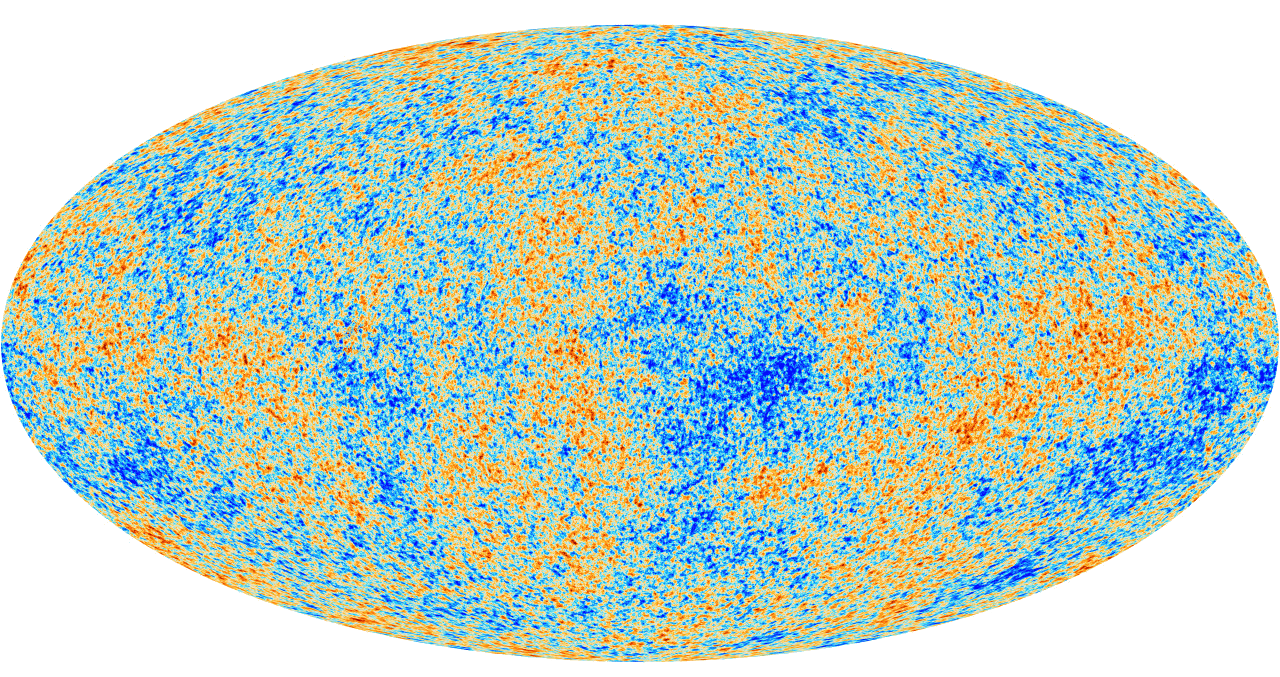
\includegraphics[scale=0.3]{cmb2019}\\
     \tiny{The Cosmic Microwave Background - as seen by Planck. Credit: ESA and the Planck Collaboration}
  \end{figure}

% \small 
%   Why was the temperature of the CMB the same in all directions? \\
%   What was the origin of the small temperature fluctions?
  
\end{frame}


\begin{frame}
      \begin{figure}
    \centering
    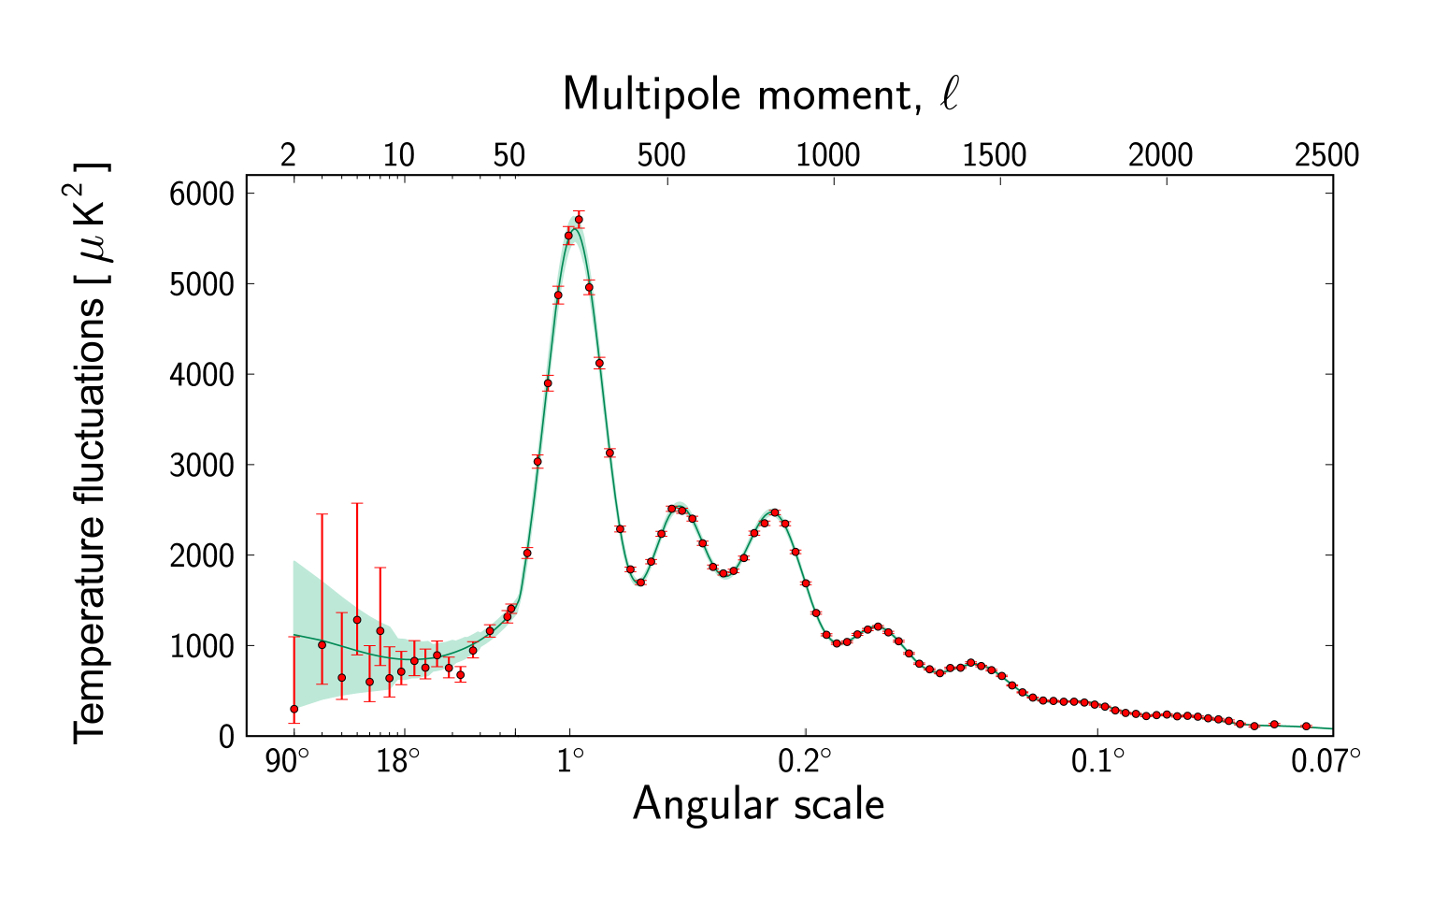
\includegraphics[scale=1]{planck2019}\\
     \tiny{Planck's power spectrum of temperature fluctuations, $\Delta T$, in the Cosmic Microwave Background. Credit: ESA and the Planck Collaboration}
  \end{figure}

% \small 
%   Why was the temperature of the CMB the same in all directions? \\
%   What was the origin of the small temperature fluctions?
  
\end{frame}



\begin{frame}
\begin{columns}
  \begin{column}{0.3\textwidth}
    \begin{block}{{\color{magenta}$\Lambda$}CDM: $\Omega=1$, $\color{magenta}w=-1{}^{\dagger}$}
     \rowcolors{1}{RoyalBlue!20}{}
      \begin{tabular}{l|c}
              Symbol& Value\\ \hline
      \color{Yellow}$\Omega_b h^2$ & \color{Yellow} $0.022\,30(14)$ \\
     \color{blue} $\Omega_{\text{CDM}} h^2$ &\color{blue} $0.1188(10)$ \\
        $t_0$ & $13.799(21)\times 10^9\, \text{years}$ \\
        $n_s$ & $0.9667(40)$\\
        $\Delta_R^2$ &$2.441\times 10^{-9}$\\
        $\tau$ & $0.066(12)$ \\
      \end{tabular}
        {\color{magenta}${}^{\dagger}${\tiny Cosmological constant}}
    \end{block}
  \end{column}
  \begin{column}{0.7\textwidth}
          \begin{figure}
    \centering
    \only<1>{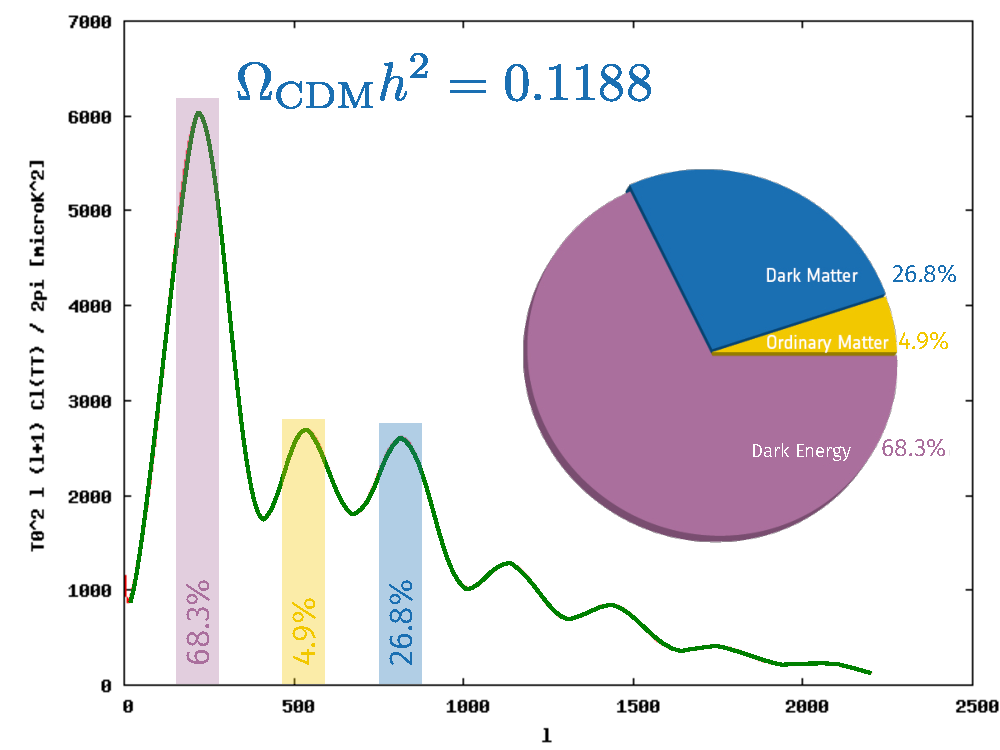
\includegraphics[scale=0.6]{cmbsoup0}}%
    \only<2>{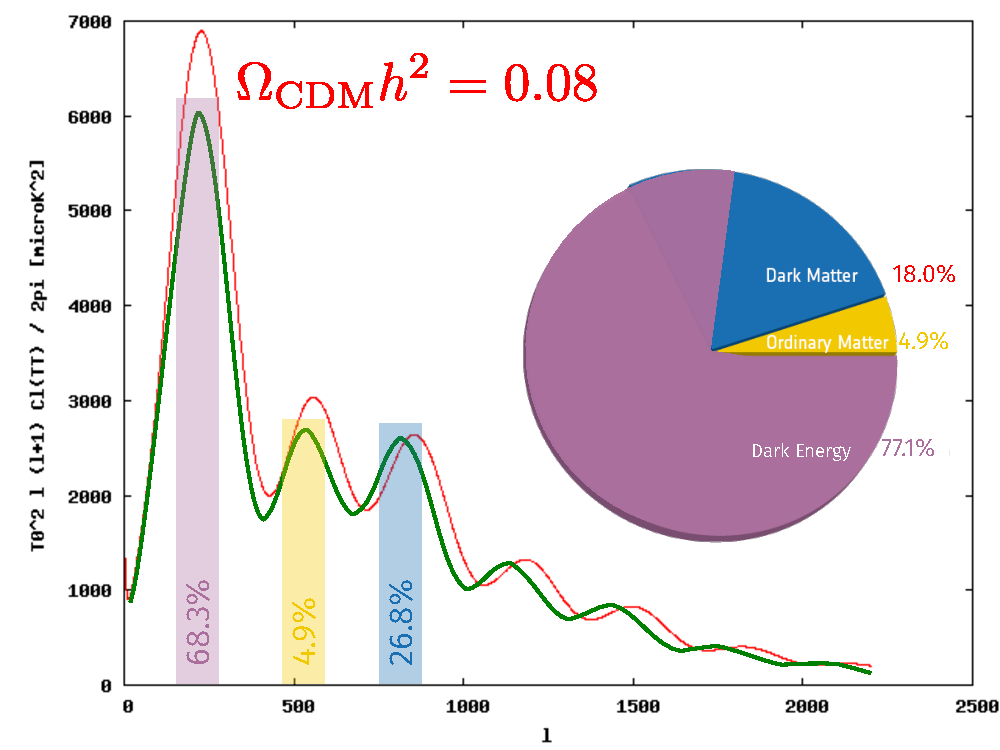
\includegraphics[scale=0.6]{cmbsoup1}}\\
    % \tiny{Credit: Planck 2018}
  \end{figure}
  \end{column}
\end{columns}
\end{frame}




\begin{frame}
\begin{picture}(320,250)  
  % \def\sdm{0.4}
  \only<1>{\put(35,-22){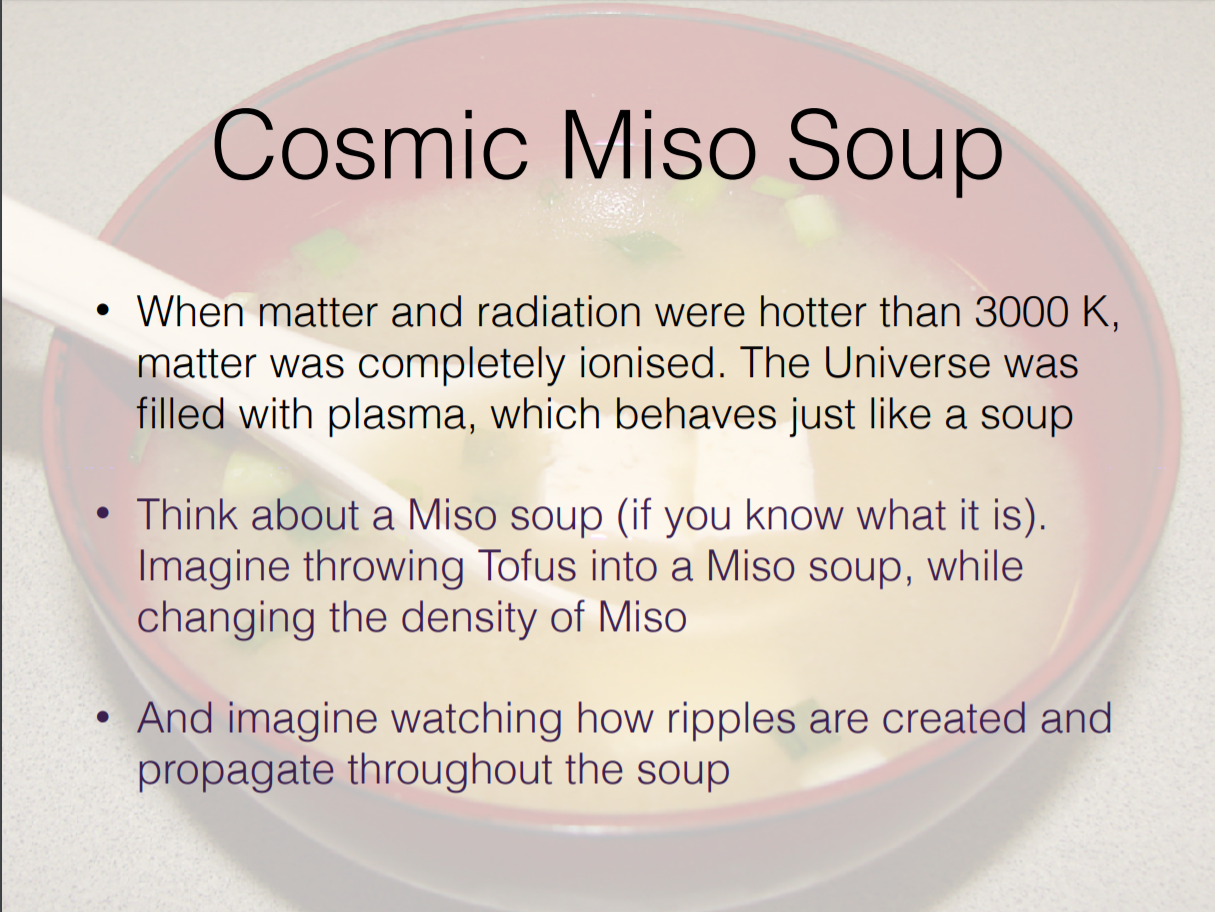
\includegraphics[height=\paperheight]{soup}}}%
  %\only<2>{\put(35,-22){
\includegraphics[height=\paperheight]{soup1}}}%
  \only<2>{\put(35,-22){
\includegraphics[height=\paperheight]{saosoup}}}%
  \only<1>{\put(235, -15){{\tiny Credit: Komatsu, ICTP Summer School on Cosmology 2018 {\tiny (Video avalaible)}}}}%
    \only<2>{\put(235, -15){{\tiny \color{white} Nobu S\~ao Paulo version}}}%  

%    \only<1>{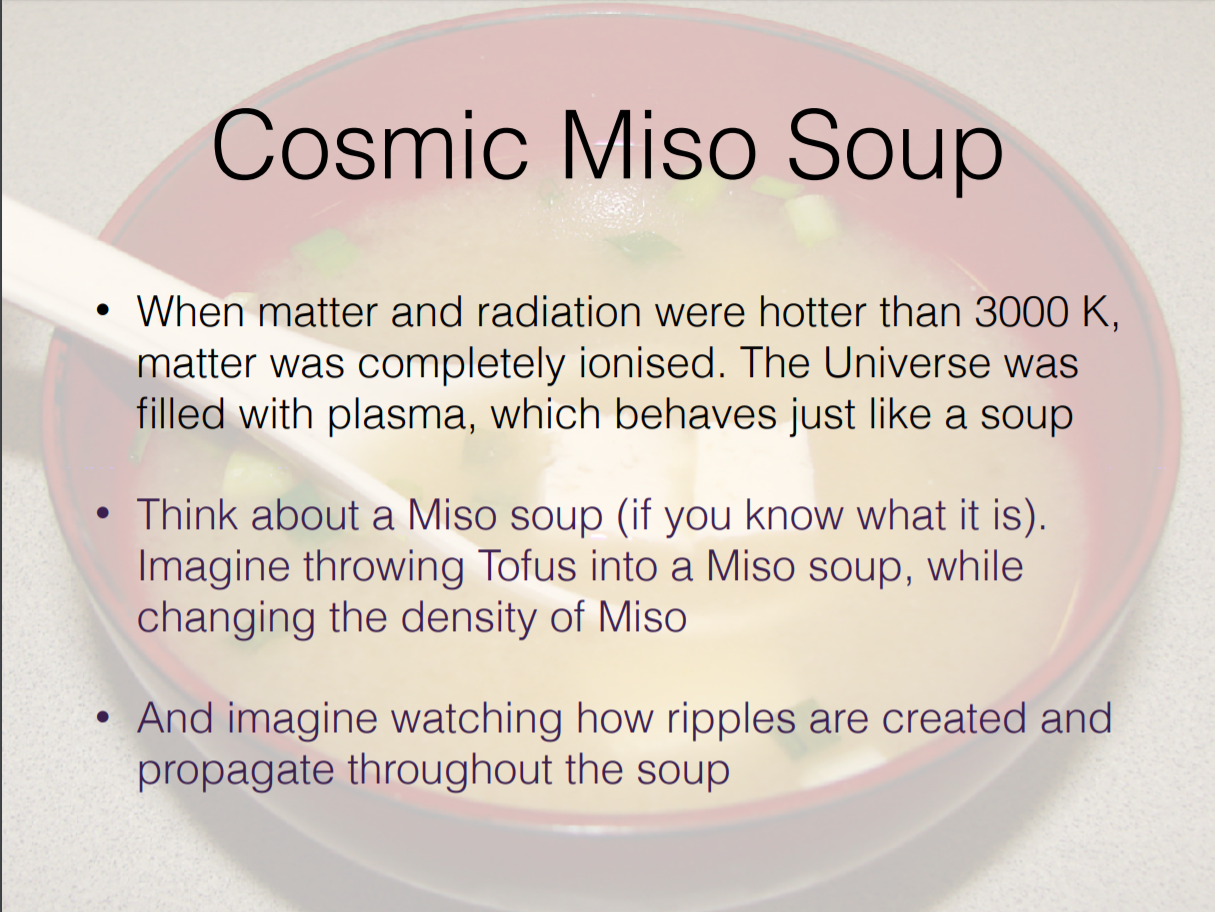
\includegraphics[scale=\sdm]{soup}}%
%    \only<2>{
\includegraphics[scale=\sdm]{soup1}}\\
%    \only<1->
\end{picture}

\end{frame}



\begin{frame}
  \frametitle{Large scale structure simulations: \small Gas of not hot and almost collisionless dark matter \alert{particles}}
  \begin{figure}
    \centering
    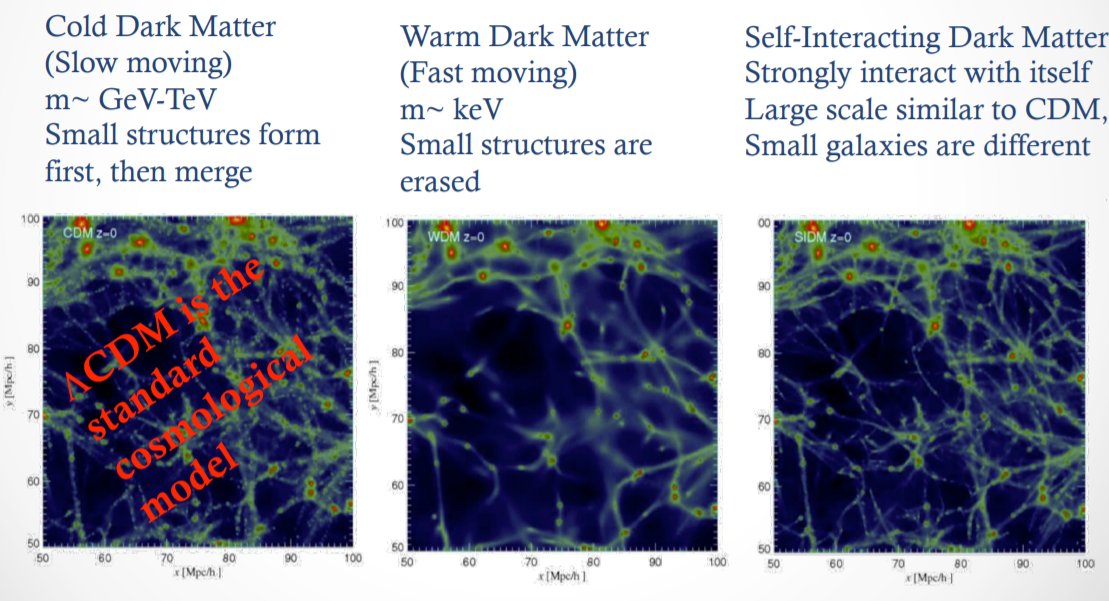
\includegraphics[scale=0.3]{dmtypes}\\
    {\tiny Credit: Arianna Di Cintio (Conference on Shedding Light on the Dark Universe with Extremely Large Telescopes, ICTP - 2018)}
  \end{figure}

\small  \alert{Particle}: from elementary sub-eV to Primordial Black Hole of several solar masses
\end{frame}


\begin{frame}
  \frametitle{Baryonic effects}
  \begin{figure}
    \centering
    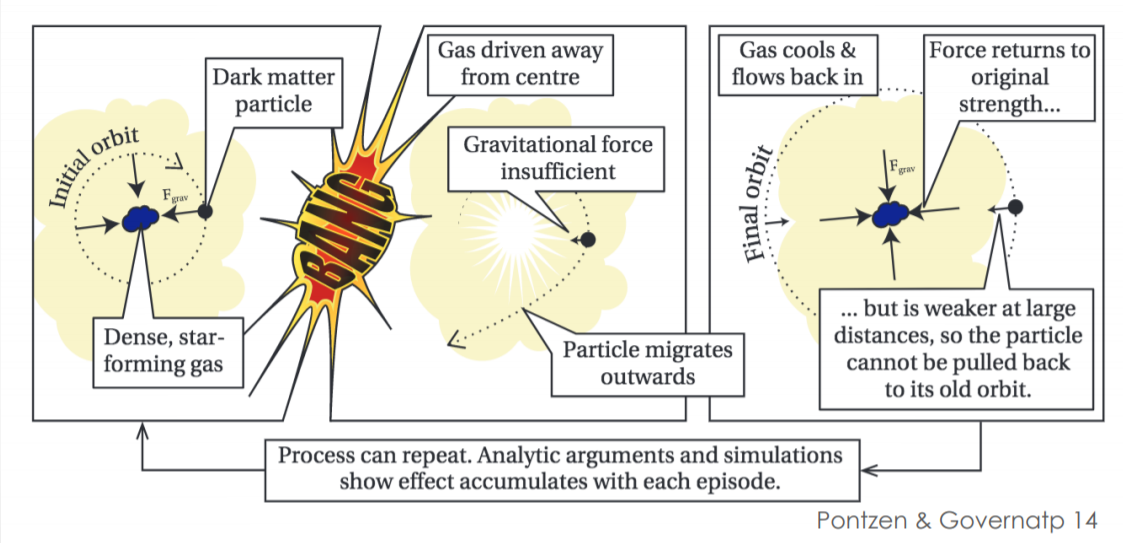
\includegraphics[scale=0.3]{snbang}
  \end{figure}
  Once the effect of baryonic physics is included, it is
  \alert{hard to distinguish between WDM/SIDM/CDM}

  \begin{center}

\vspace{-0.5cm}    
\footnotesize
\begin{itemize}
\item For a review see: Gravitational probes of dark matter physics, M.R. Buckley, \emph{et al}, arXiv:1712.06615 [PR]
\item Distinguish WDM/CDM with subhaloes detection: See \arXiv{1910.06617}
\end{itemize}

  \end{center}
\end{frame}


\begin{frame}
  \frametitle{Cosmic web}

      \alert{Dark matter} in the universe evolves through gravity to form a complex network
      of halos, filaments, sheets and voids, that is known as the cosmic web

      {\tiny A.C Rodriguez \emph{et al} arXiv:1801.09070 [CAC]}

    Cosmological simulations of structure formation predict that the
    \alert{majority of gas} in the intergalactic medium (IGM) is distributed
    in a cosmic web of sheets and filaments as a consequence of
    gravitational collapse.  The intersections of these structures
    become the locations at which galaxies and their supermassive
    black holes (SMBHs) form and evolve.

    [...] %at a $z$ of $\sim 3$,
    \alert{$60\%$ of all gas} in the
    Universe resides in filaments
    
    {\tiny H. Umehata \emph{et al}, Science  \textbf{366}, 97, 4 Oct 2019}

% Read more at: 

%   \frametitle{General considerations}
%   \note{From doi:  [10.1098/rsta.2009.0209]
%     We live in an exciting, if somewhat bewildering, time in terms of our understanding of the Universe. The concept of dark matter, as a significant component of the Universe, dates back to the 1970s following the realization that most galaxies are surrounded by unseen haloes. The null results of the Galactic microlensing surveys and the abundance of light elements produced in the big bang further suggest that dark matter is non-baryonic in form. Structure formation models can account for the presently observed large-scale distribution of galaxies if this non-baryonic matter is made of massive non-relativistic (i.e. ‘cold’) particles. Despite this progress, after 40 years, we have yet to detect the dark matter particle itself. Given how both strong and weak gravitational lensing have, in barely a decade, considerably added to our knowledge of the distribution and amount of dark matter, it is relevant to ask what these techniques can offer in the future.}

%   \note{Astronomical observations can define the spatial distribution of dark matter from small to large scales. Theory predicts this distribution in terms of the spectrum of physical scales over which the density of dark matter fluctuates. }
\end{frame}

% \begin{frame}
%   \frametitle{Galaxy catalogs}
%   \begin{columns}
%   \begin{column}{0.65\textwidth}
%   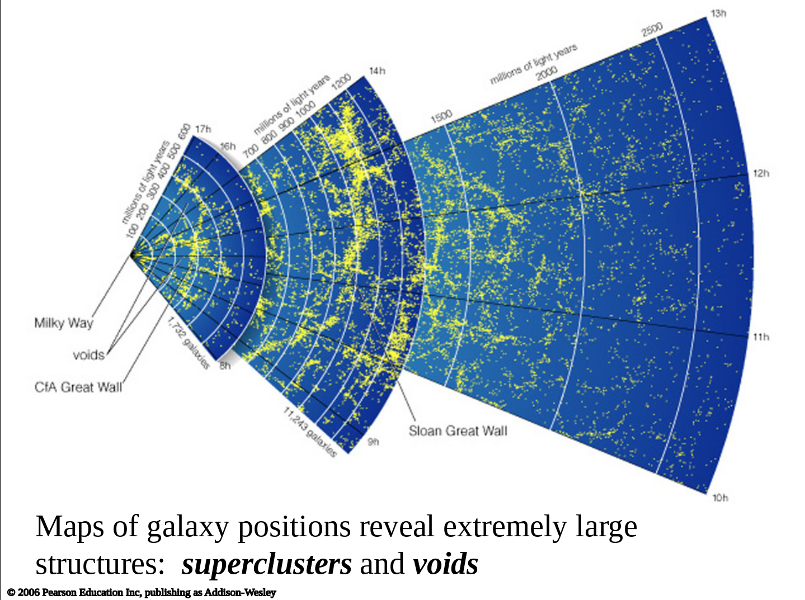
\includegraphics[scale=0.35]{galaxsmall}     
%   \end{column}
%   \begin{column}{0.35\textwidth}
%     The DESI experiment\\
%     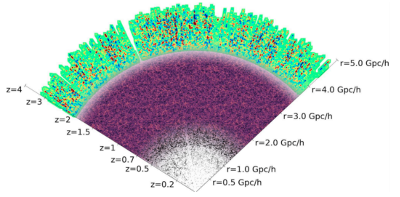
\includegraphics[scale=0.43]{DESIsmall}
    
%     {\tiny Credits: J. Forero \url{http://cosmology.univalle.edu.co/} }
%   \end{column}
% \end{columns}

%   %\vspace{-0.3cm}

% \end{frame}



\begin{frame}
  \frametitle{Cooking the soup: Cosmic web}
  \begin{quote}
    Dark matter connects clusters of galaxies with massive tendrils, forming a cosmic web that serves as an unseen skeleton for the universe.

\vspace{-0.3cm}    
    {\tiny \url{https://phys.org/news/2018-06-years-scientists-account-universe.html}}

    
  \end{quote}

\def\heifig{3.8cm}
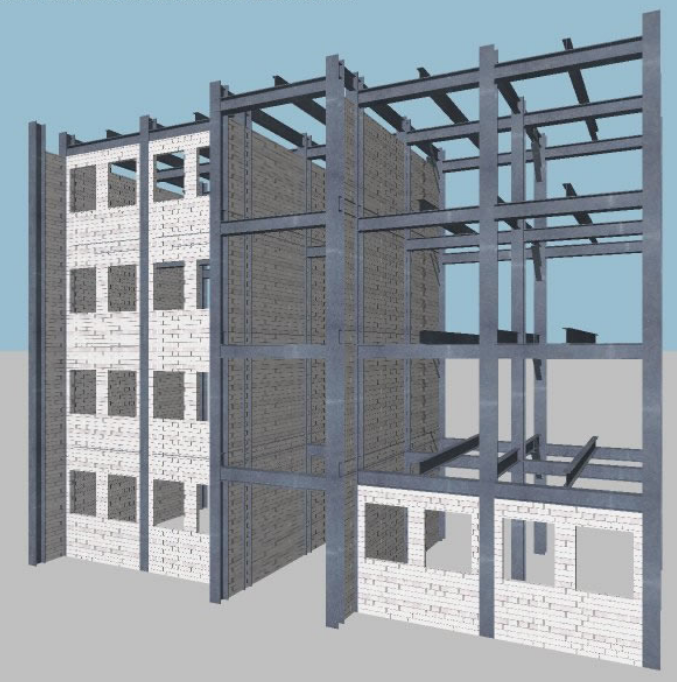
\includegraphics[height=\heifig]{building} \hfill \only<1-2>{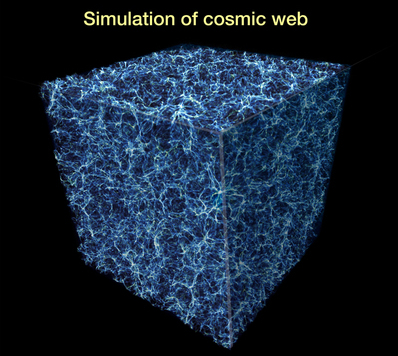
\includegraphics[height=\heifig]{lowweb}}\only<3>{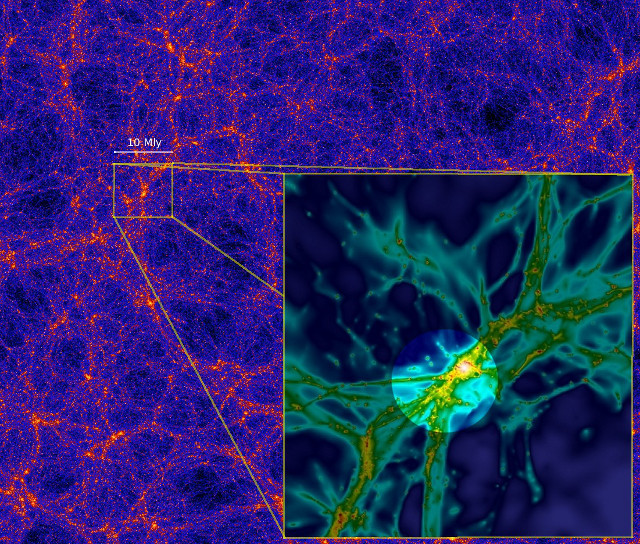
\includegraphics[height=\heifig]{cosmic_web_simulation}}

  % \begin{figure}
  %   \centering
  %   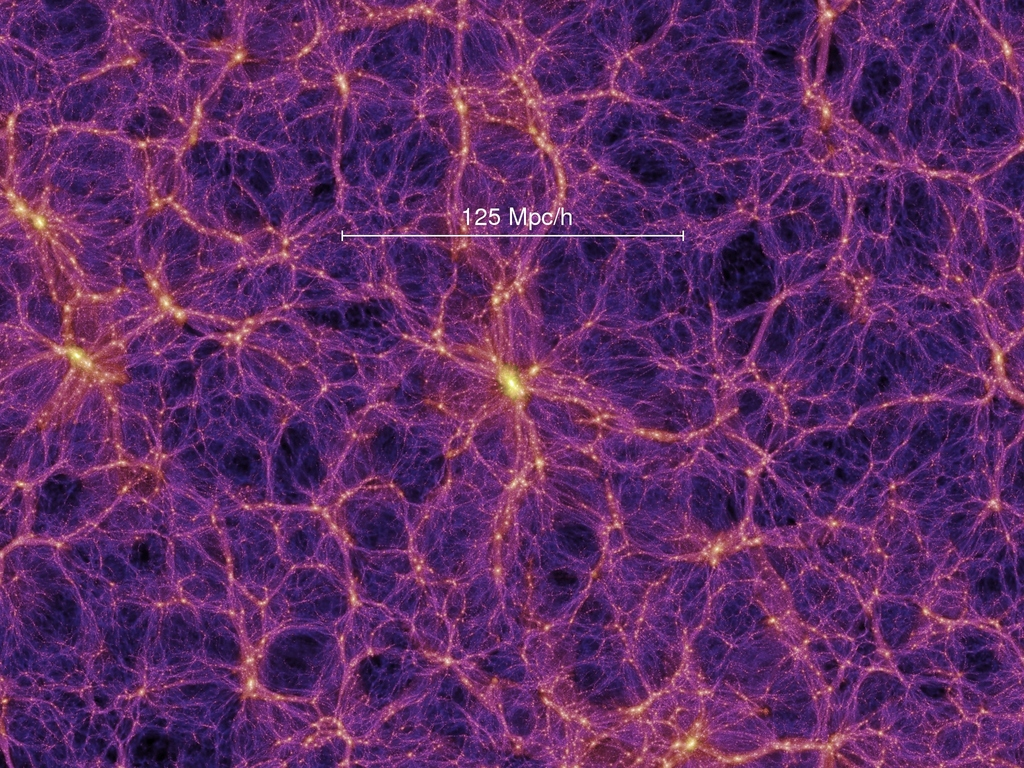
\includegraphics[scale=0.2]{cosmic-web}\\
  %   {\tiny Milenium simulation: \url{https://wwwmpa.mpa-garching.mpg.de/galform/virgo/millennium/}}
  % \end{figure}
\only<1-3>{
\invisible<1-2>{
{  \scriptsize These great filaments are made largely of \alert{dark matter} located in the space between galaxies\\ and filled with $60\%$ of the \alert{primordial gas!} \hfill\only<1>{{[\url{https://hubblesite.org}]}}
}

%\vspace{-0.3cm}
\begin{block}{\footnotesize An excess of a gas ($20\sigma$) is observed between Milky Way and Andromeda (M31): arXiv:1403.7528 [MNRAS] ${}^1$} 
  \footnotesize Clouds of HI likeky embeded in a filament between M31 and M33: arXiv:1305.1631 [nature]\\ 
\end{block}

\vspace{-0.3cm}
{\tiny $\overline{{}^1\ \ \ \ \ \ }$\!\!\!\!\!\!\!See also: arXiv:1603.05400 [A\&A]}
}
}
\begin{picture}(320,10)
  \only<2>{ \put(30,80){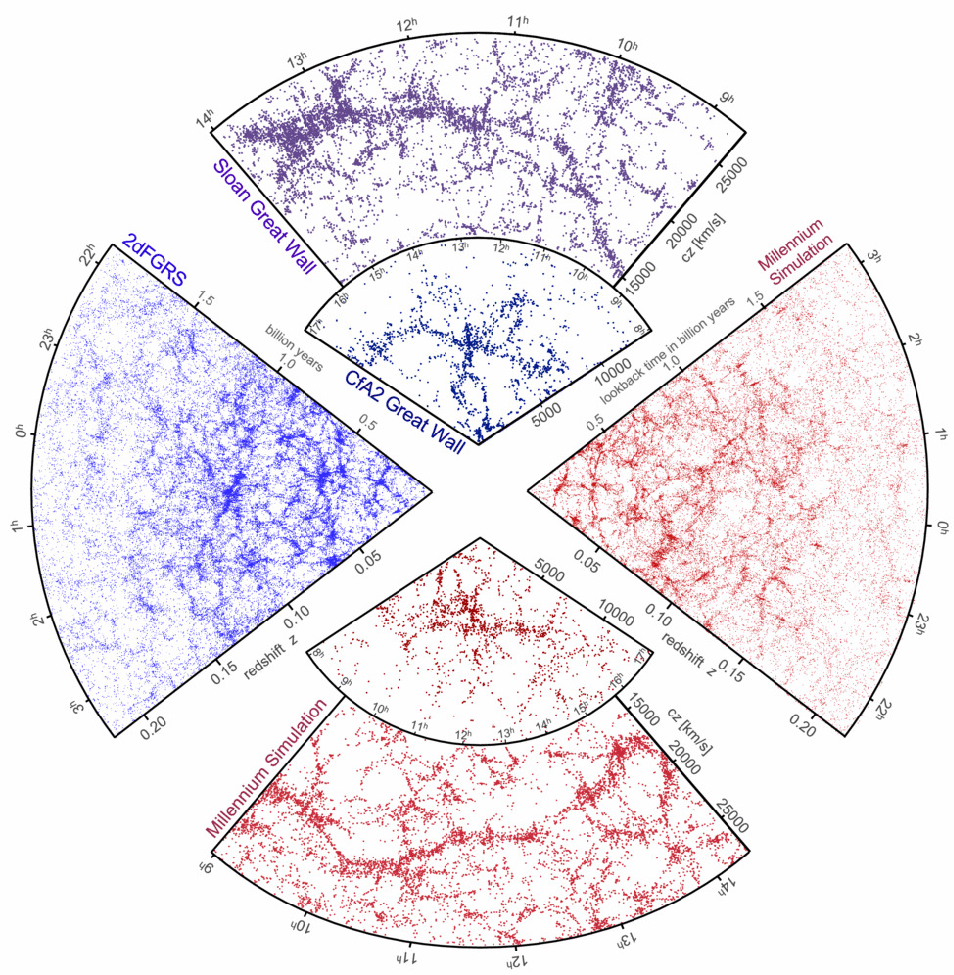
\includegraphics[scale=0.3]{fig1_lowres}} }
  \only<2>{ \put(-60,70){{\tiny Galaxy redshift surveys vs large scale structure formation simulations: V. Springel, \emph{et al} \texttt{astro-ph/0604561} [Nature]}} }
\end{picture}
\end{frame}


% % \begin{frame}
% %   \frametitle{Cosmic Anatomy}
% %   \def\sana{0.8cm}
% %   \centering
% %   { \tiny Baryons \hspace{\sana} Missing Baryons \hspace{\sana} Dark Matter}
% %   \begin{figure}
% %     \centering
% %     
\includegraphics[scale=0.6]{anatomy}\\
% %   \end{figure}
% % \end{frame}


% % \begin{frame}
% %     \frametitle{The muscles}
% % \begin{figure}
% %   \centering
% %   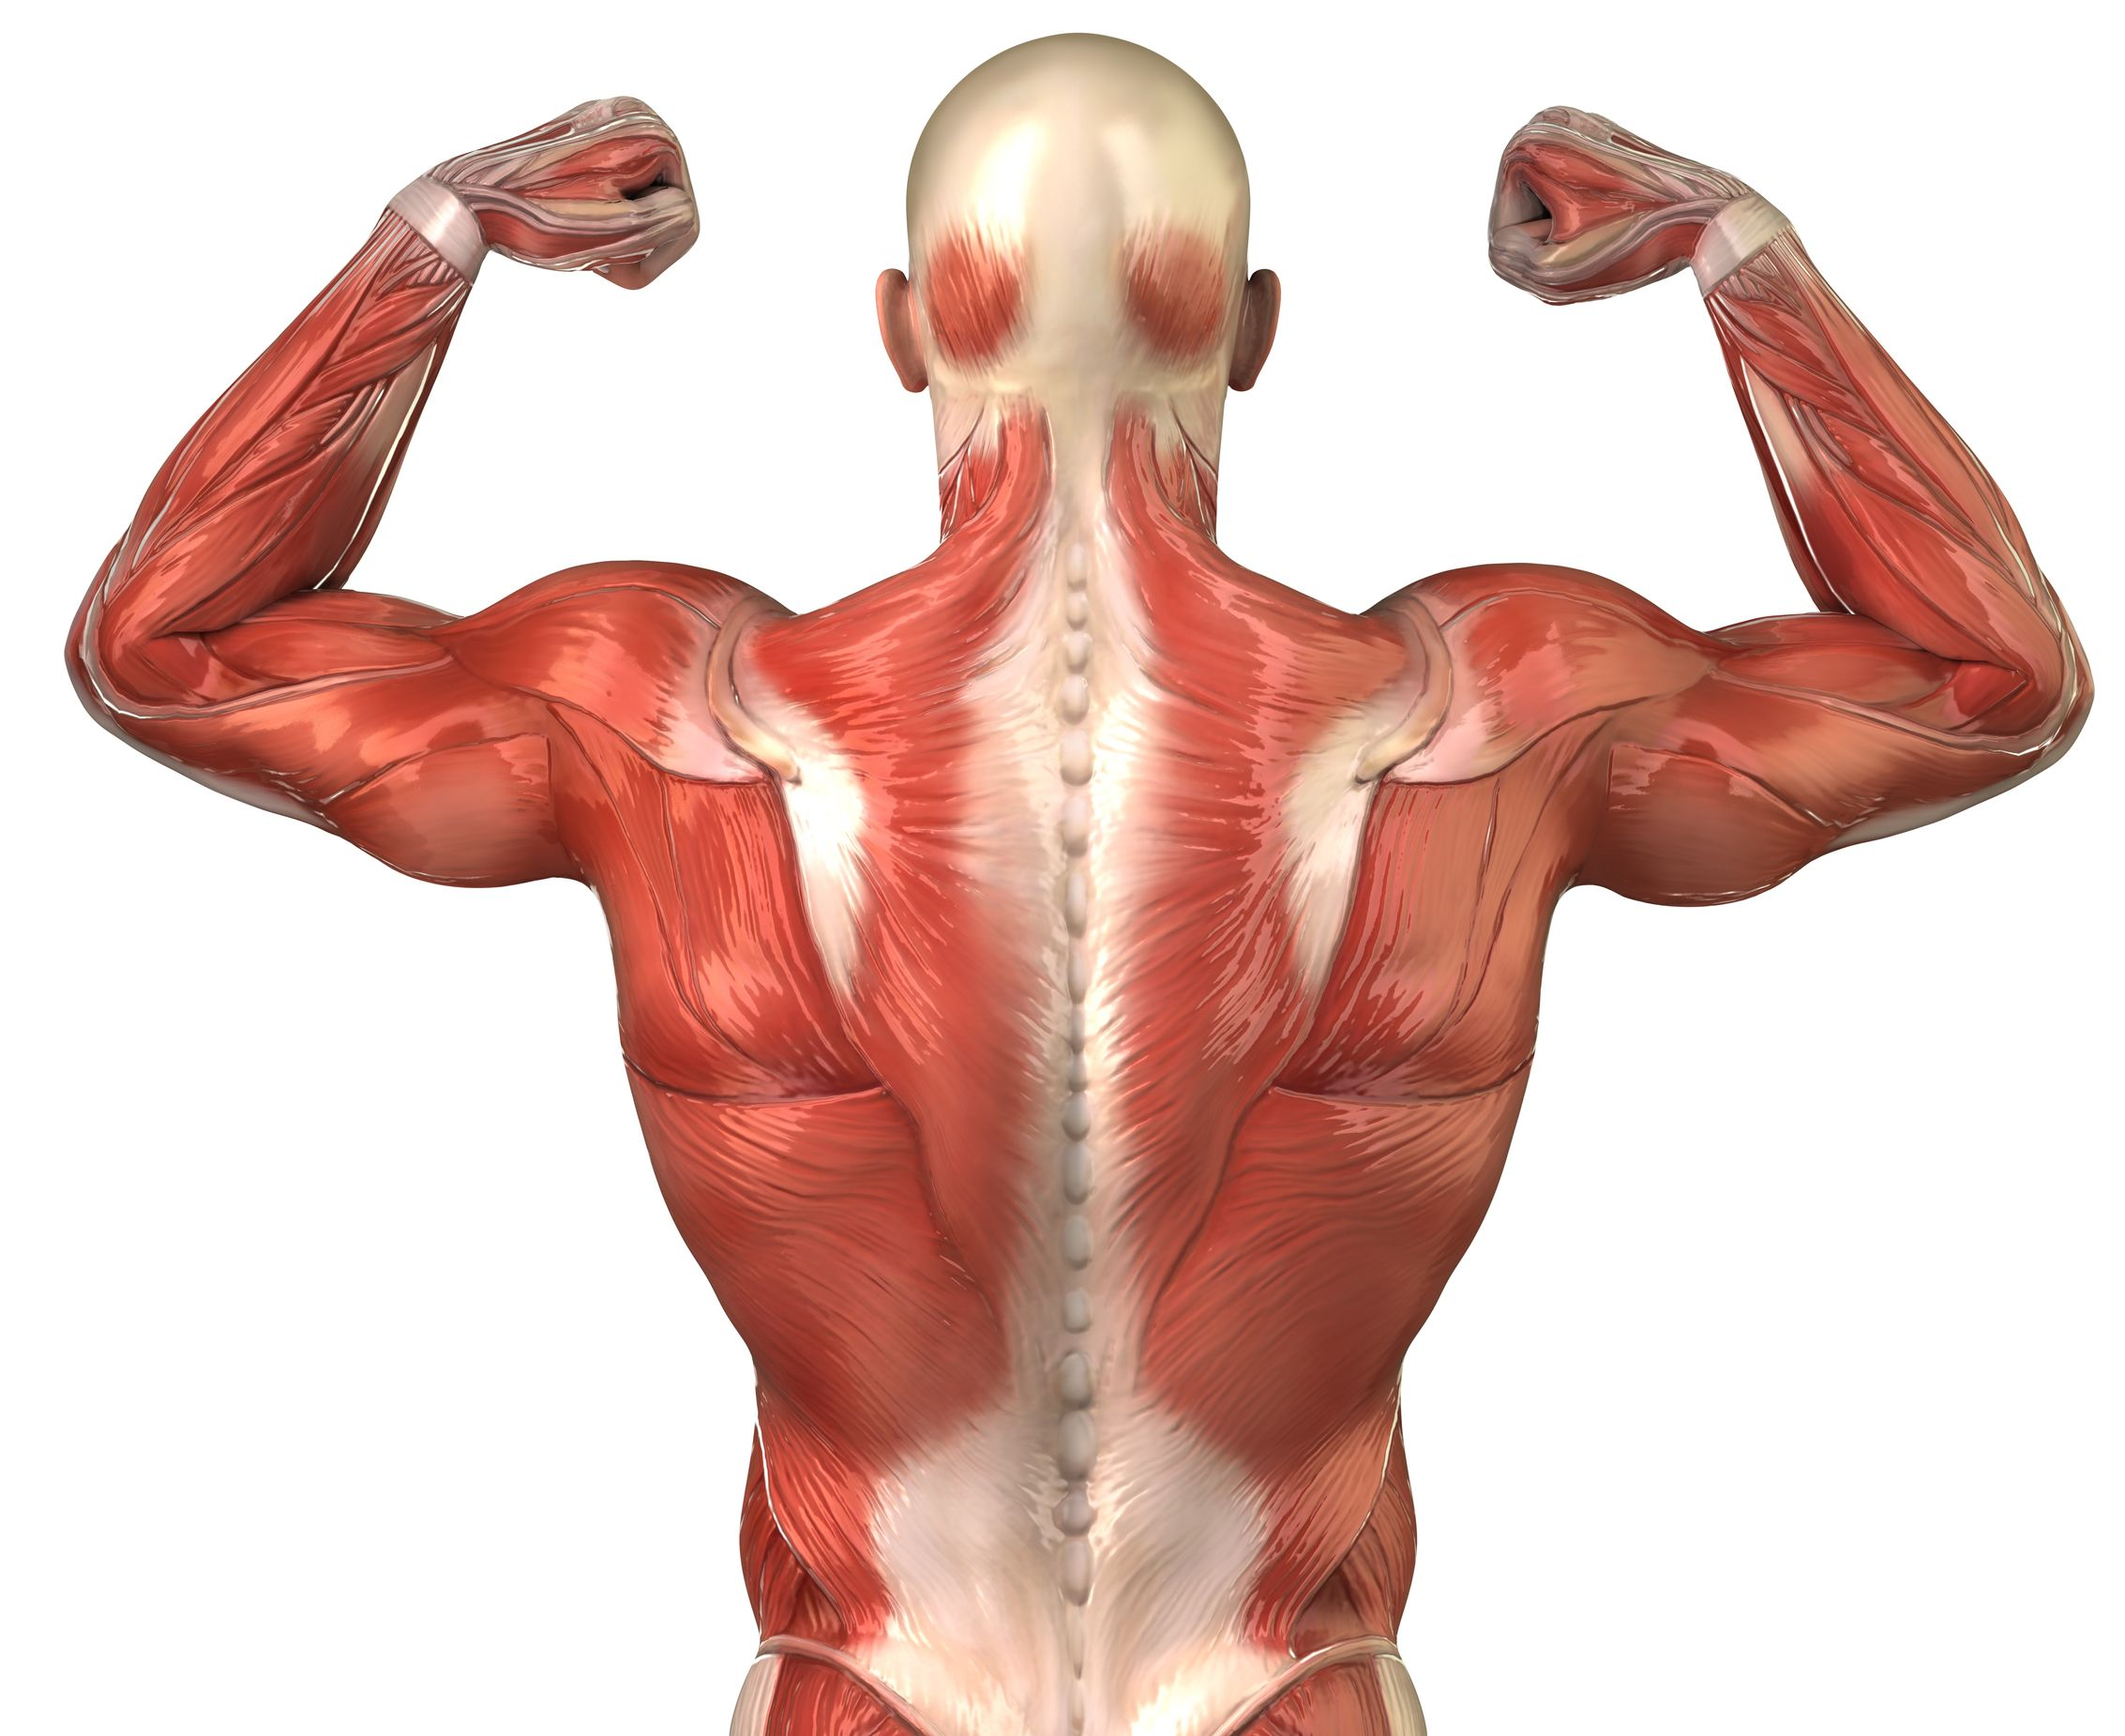
\includegraphics[scale=0.5]{muscles-anatomy-back}\\
% %   {\tiny Credit: \url{http://sciencedrivennutrition.com}}
% % \end{figure}
% % \end{frame}

\begin{frame}
  \frametitle{Direct observations of filaments}
  \small
  \textbf{Where are the Baryons?} (Cen, Ostriker, astro-ph/9806281 [AJ])
  \begin{quote}
   \scriptsize Thus, not only is the universe dominated by dark matter, but more than one half of the normal matter is yet to be detected. (the muscles)
  \end{quote}

  \vspace{-0.5cm}

\begin{columns}
  \begin{column}{0.48\textwidth}
\begin{figure}
  \centering
  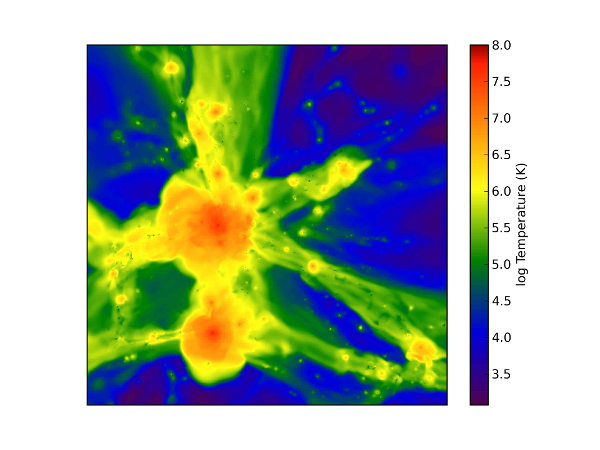
\includegraphics[scale=1.4]{clusterboXsmall}\\
  {\tiny Credit: Cen, arXiv:1112.4527 [AJ]}
\end{figure}

  \end{column}
  \begin{column}{0.48\textwidth}
    \scriptsize
    Warm-hot intergalactic medium (WHIM)

    Density-weighted temperature projection of a portion of the refinement box of the C run of size  $\left(18\,h^{-1}\text{Mpc} \right)^3$.

    Low temperature WHIM confirmed by O VI line that peak at $T\sim 3\times 10^5\ \text{K}$
  \end{column}
\end{columns}

\small   

\includegraphics[scale=0.1]{new}Hotter phases of the WHIM: \textbf{  Observations of the missing baryons in the warm-hot intergalactic medium}
  (Nicastro, \emph{et al.} arXiv:1806.08395 [Nature]). 

\end{frame}


% umerical simulations in the framework of the commonly accepted (ΛCDM) cosmological paradigm predict that, starting at a redshift of $z\approx 2$ and during the continuous process of structure formation, diffuse baryons in the intergalactic medium (IGM) condense into a filamen-tary web (with electron densities of $n_e\approx 10^{-6}-10^{-4}\ \text{cm}^{-3}$ and undergo shocks that heat them up to temperatures of $T\approx 10^5-10^7\ \text{K}$, making the by-far-largest constituent of the IGM, hydrogen, mostly ionized. At the same time, galactic outflows powered by stellar and active galactic nucleus (AGN) feedback enrich the IGM baryons with metal. How far from galaxies these metals roam depends on the energetics of these winds, but it is expected that metals and galaxies are spatially correlated.
  
  %     \begin{quote}
  % From: \url{https://phys.org/news/2018-06-years-scientists-account-universe.html}

  %   The scientists used the European Space Agency's XMM-Newton X-ray space telescope to study the BL Lacertae quasar 1ES 1553+113, an active, supermassive black hole at the center of a galaxy. Quasars gobble up matter and shine brightly in many wavelengths of light, from radio waves to X-rays. These celestial lighthouses can basically back light the material that crosses the beam's path, just as a flashlight beam illuminates unseen motes of dust in the air.
  % \end{quote}

  % \begin{quote}

  %   Studying the chemical fingerprint of oxygen in the X-rays from the quasar light, the scientists found a large amount of extremely hot intergalactic gas so much that they calculate that this gas could account for up to 40 percent of the baryonic matter in the cosmos, which could be enough to explain the missing matter.

  % \end{quote}

  % \begin{quote}

  %   Taotao Fang of the Jiujiang Research Institute in China, who was not involved in the study, pointed to a few possible alternate explanations, including that the ionized gas signal may have come from within a galaxy rather than from intergalactic gas embedded in a dark matter filament.
  % \end{quote}
  



% \begin{frame}
%     \frametitle{The skeleton}
% \begin{figure}
%   \centering
%   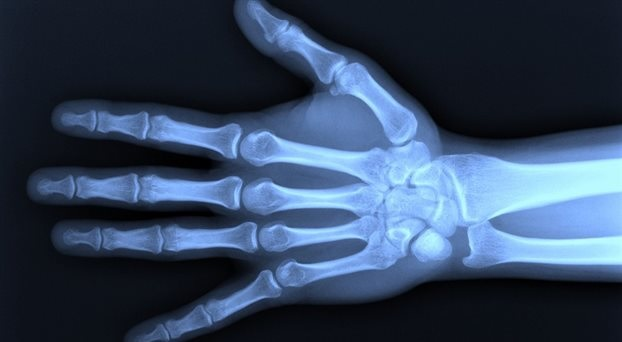
\includegraphics[scale=0.5]{xray}\\
%   {\tiny Credit: \url{https://www.disnola.com}}
% \end{figure}
% \end{frame}







% From: \url{http://www2.cnrs.fr/en/1247.htm},  
% \begin{quote}
%   the MegaCam, which has 340 megapixels, using a technique known as  “This technique works somewhat like an X-ray,” says Kilbinger. “You can’t see inside the human body, and we can’t see the dark matter directly.” Dark matter is dark, but any light emitted from galaxies must pass around it, and the diversion is recorded as a gravitational distortion. Astronomers can then use this gravitational imprint to calculate the size of the matter that caused it. Using such techniques, astronomers estimate that dark matter forms web-like structures, made up of clusters, filaments, and large rope-like structures that the new research has uncovered. But only until dark matter becomes visible will these assumptions become fact. Nonetheless, the new findings open up a dizzying vista of possibility, where, with better telescopes in the future, more precise lay-out and details of dark matter could be revealed. Understanding the formation of dark matter could help scientists improve their knowledge on how the universe evolved, and what its future might be. “There are other techniques that can measure dark matter,” says Kilbinger, “but over the next 10 to 20 years, I think this one will become the most used. And that’s why people are so excited about it.”
% \end{quote}


% From:
% \begin{quote}
%   Looking deep into space, and literally peering back in time, is like experiencing the universe in a house of mirrors where everything is distorted through a phenomenon called gravitational lensing. 
% \end{quote}



% coupled with the angular resolution of ELTs this will open a unique window to constrain the
% dark matter properties with detail and statistical completeness. 










% \begin{frame}
%   \frametitle{Evidences at all redshifts.}
% \begin{columns}
%   \begin{column}{0.48\textwidth}
%       \begin{itemize}
%   \item   For cluster of Galaxies
%   \item For stars inside Galaxies
%   \item Inside our Galaxy
%   \item Senatore reconstruction
%   \item En las simulaciones se parte de la CMB
%   \end{itemize}
%   \end{column}
%   \begin{column}{0.48\textwidth}

%       \begin{figure}
%     \centering
%     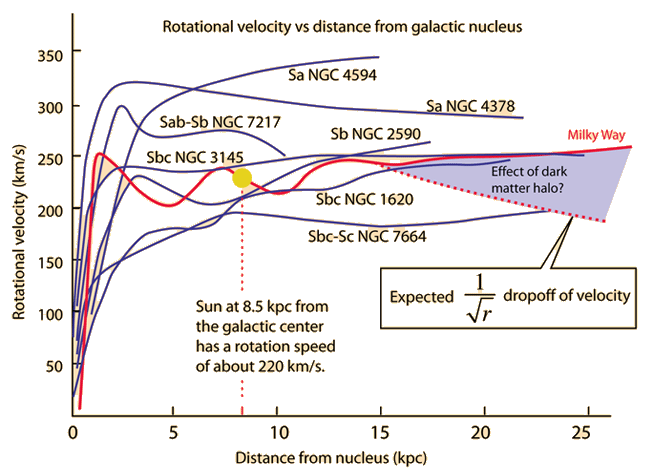
\includegraphics[scale=0.2]{gallightcrv}
%   \end{figure}

%   \end{column}
% \end{columns}

% \end{frame}



% \begin{frame}
%   \frametitle{Inner Milky Way}
%   \url{https://www.nature.com/articles/nphys3237}
% \end{frame}

\begin{frame}
  \frametitle{A filament of dark matter between two clusters of galaxies}
  \begin{columns}
  \begin{column}{0.45\textwidth}
  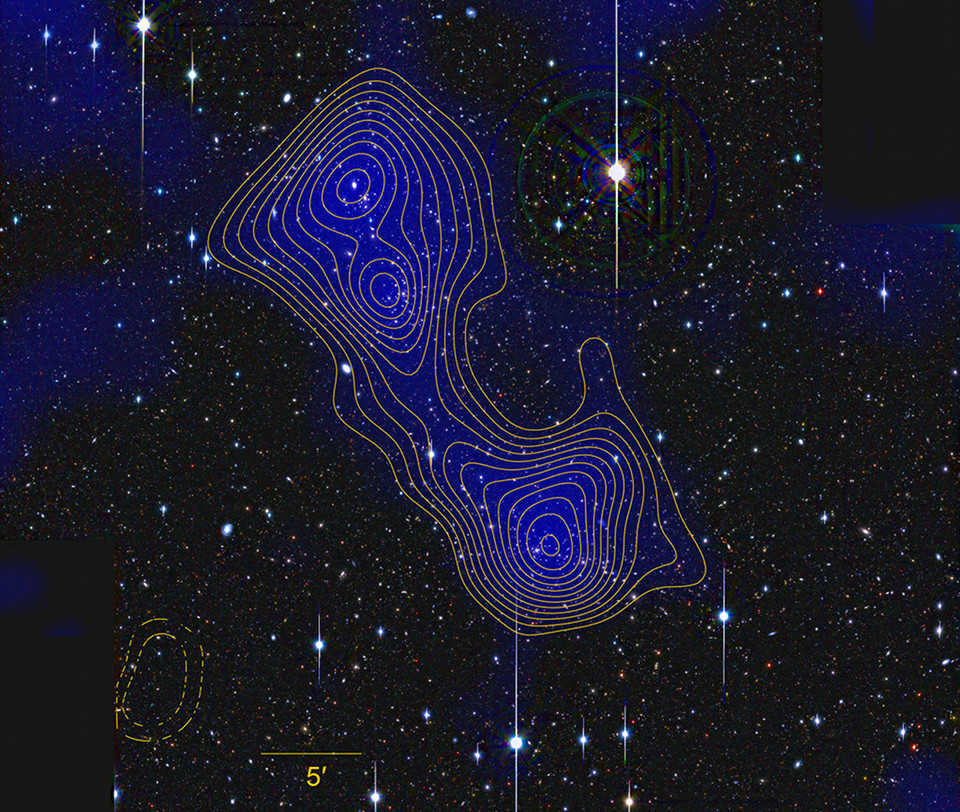
\includegraphics[height=6cm]{A222+3_mass}
  \end{column}
  \begin{column}{0.55\textwidth}
%It is a firm prediction of the concordance Cold Dark Matter (CDM) cosmological model that
%galaxy clusters live at the intersection of large-scale structure filaments

    \begin{block}{Supercluster
system of three galaxy clusters}
    \begin{itemize}
    \item Abell 222 (south) detected at $\sim 8\sigma$
    \item Abell 223 (north) double galaxy cluster seen at $\sim 7\sigma$   
    \end{itemize}

    \end{block}



  \fcolorbox{blue}{blue}{\color{white}reconstructed surface mass density (blue)}
  
  \fcolorbox{Yellow}{white}{significance contours from $0.5\sigma$ to $2.5\sigma$}


    {\tiny J.P. Dietrich \emph{et al}, arXiv:1207.0809 [Nature]}

   {\tiny For a recent review see: arXiv:1905.08991}  
  \end{column}
  \end{columns}

\end{frame}

\begin{frame}
  \frametitle{Three-dimensional pictures of Ly$\alpha$ filaments}
  \begin{columns}
  \begin{column}{0.5\textwidth}
  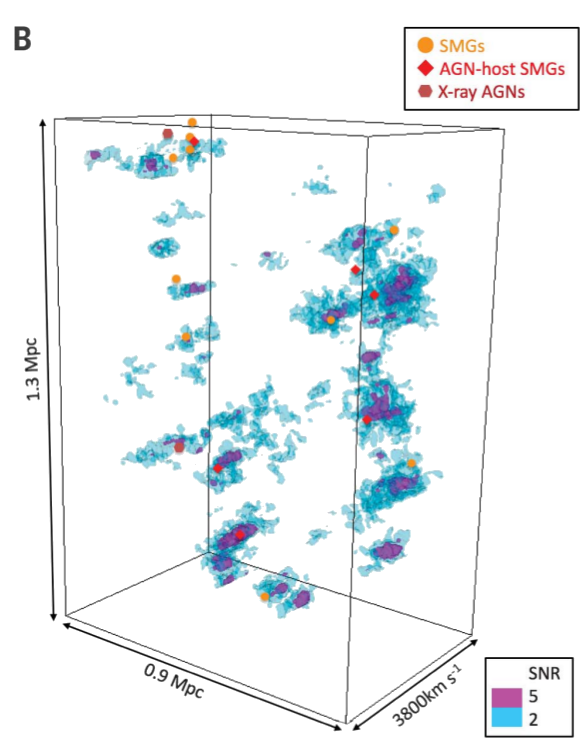
\includegraphics[scale=0.3]{fila}
  \end{column}
  \begin{column}{0.5\textwidth}
  The 3D distribution of
  Ly$\alpha$ filaments shown with

  \fcolorbox{magenta}{magenta}{signal-to-noise ratio (SNR) > 5}
  
  \fcolorbox{cyan}{cyan}{signal-to-noise ratio (SNR) > 2}


    {\tiny H. Umehata \emph{et al}, Science  \textbf{366}, 97, \alert{4 Oct 2019}}

  \end{column}
  \end{columns}

\end{frame}